% 理论部分独立稿：保留完整论文第 1--5 节，不包含第 6 节起的数值实验与附录。
% 编译顺序：xelatex -> biber -> xelatex -> xelatex。
%!TEX program = xelatex
\documentclass[lang=cn,a4paper,newtx]{elegantpaper}

\title{ICU约束下基于隔离率的流行病阈值控制策略分析}
\author{ XXX \and XXX}
\institute{School of Mathematics and Statistics, Shaanxi Normal University}
% \version{0.1}
\date{}

\usepackage{amsmath,amssymb,mathrsfs}
\usepackage{booktabs}
\usepackage{graphicx}
\usepackage{float}
\usepackage{placeins}
\usepackage{array}
\usepackage{tabularx}
\usepackage{multirow}
\usepackage{makecell}
\usepackage{threeparttable}
\usepackage{siunitx}
\usepackage{xurl}
\usepackage{algorithm}
\usepackage{algpseudocode}

\graphicspath{{./}{figures/}{table/}}
\numberwithin{equation}{section}
% 推论与定理共用编号。
\theoremstyle{plain}
\newtheorem{corollaryn}[theorem]{推论}
% 需要交叉引用的注记采用编号环境。
\newtheorem{remarkn}[theorem]{注记}
\allowdisplaybreaks[3]
\renewcommand{\arraystretch}{1.12}
\emergencystretch=2em
\newcommand{\qinf}{q_{\mathrm{inf}}}
\newcommand{\Itcum}{I_{t_{\mathrm{cum}}}}
\addbibresource{references.bib}

\begin{document}

\maketitle

\begin{abstract}
\textit{（摘要待撰写。）}
\end{abstract}

\section{引言}
\textit{（引言与文献综述待撰写。）}

\section{模型与阈值控制策略}
\label{sec:model}
\subsection{包含接触追踪与隔离的扩展 SIR 型模型}
将人群分为易感者（$S$）、隔离易感者（$S_q$）、非隔离感染者（$I$）、隔离感染者（$I_q$）和康复者（$R$）五个仓室。记传播概率为 $\beta$，接触率为 $c(t)$，接触追踪比例为 $q(t)$。被追踪到的接触者中，未感染者进入 $S_q$，感染者进入 $I_q$；未被追踪到的接触者占比为 $1-q(t)$，其中感染者进入 $I$。非隔离感染者和隔离感染者分别以速率 $\gamma$ 和 $\delta_q$ 康复，并进入 $R$。

该模型为含接触追踪与隔离的扩展 SIR 型模型，下文简称 SIQR 型模型，其方程为


\begin{equation}
\begin{cases}
\dfrac{dS(t)}{dt} = -\dfrac{\beta c(t) + c(t)q(t)(1-\beta)}{N} S(t)I(t), \\[.8em] % Add some space after the first line
\dfrac{dI(t)}{dt} = \dfrac{\beta c(t)(1-q(t))}{N} S(t)I(t)  - \gamma I(t), \\[.8em]
\dfrac{dS_q(t)}{dt} = \dfrac{(1-\beta)c(t)q(t)}{N} S(t)I(t), \\[.8em]
\dfrac{dI_q(t)}{dt} = \dfrac{\beta c(t) q(t)}{N} S(t)I(t) - \delta_q I_q(t), \\[.8em]
\dfrac{dR(t)}{dt} = \gamma I(t) + \delta_q I_q(t).
\end{cases}
\label{eq:model:full}
\end{equation}

式~\eqref{eq:model:full} 中，$q(t)$ 同时影响新感染者进入 $I$ 与 $I_q$ 的比例，以及易感者进入隔离的数量。因此，即使接触率保持不变，调整隔离率仍会同时改变 $S$ 和 $I$ 的演化。相应的仓室转移结构见图~\ref{fig:model_schematic}。

\begin{figure}[htbp]
    \centering
    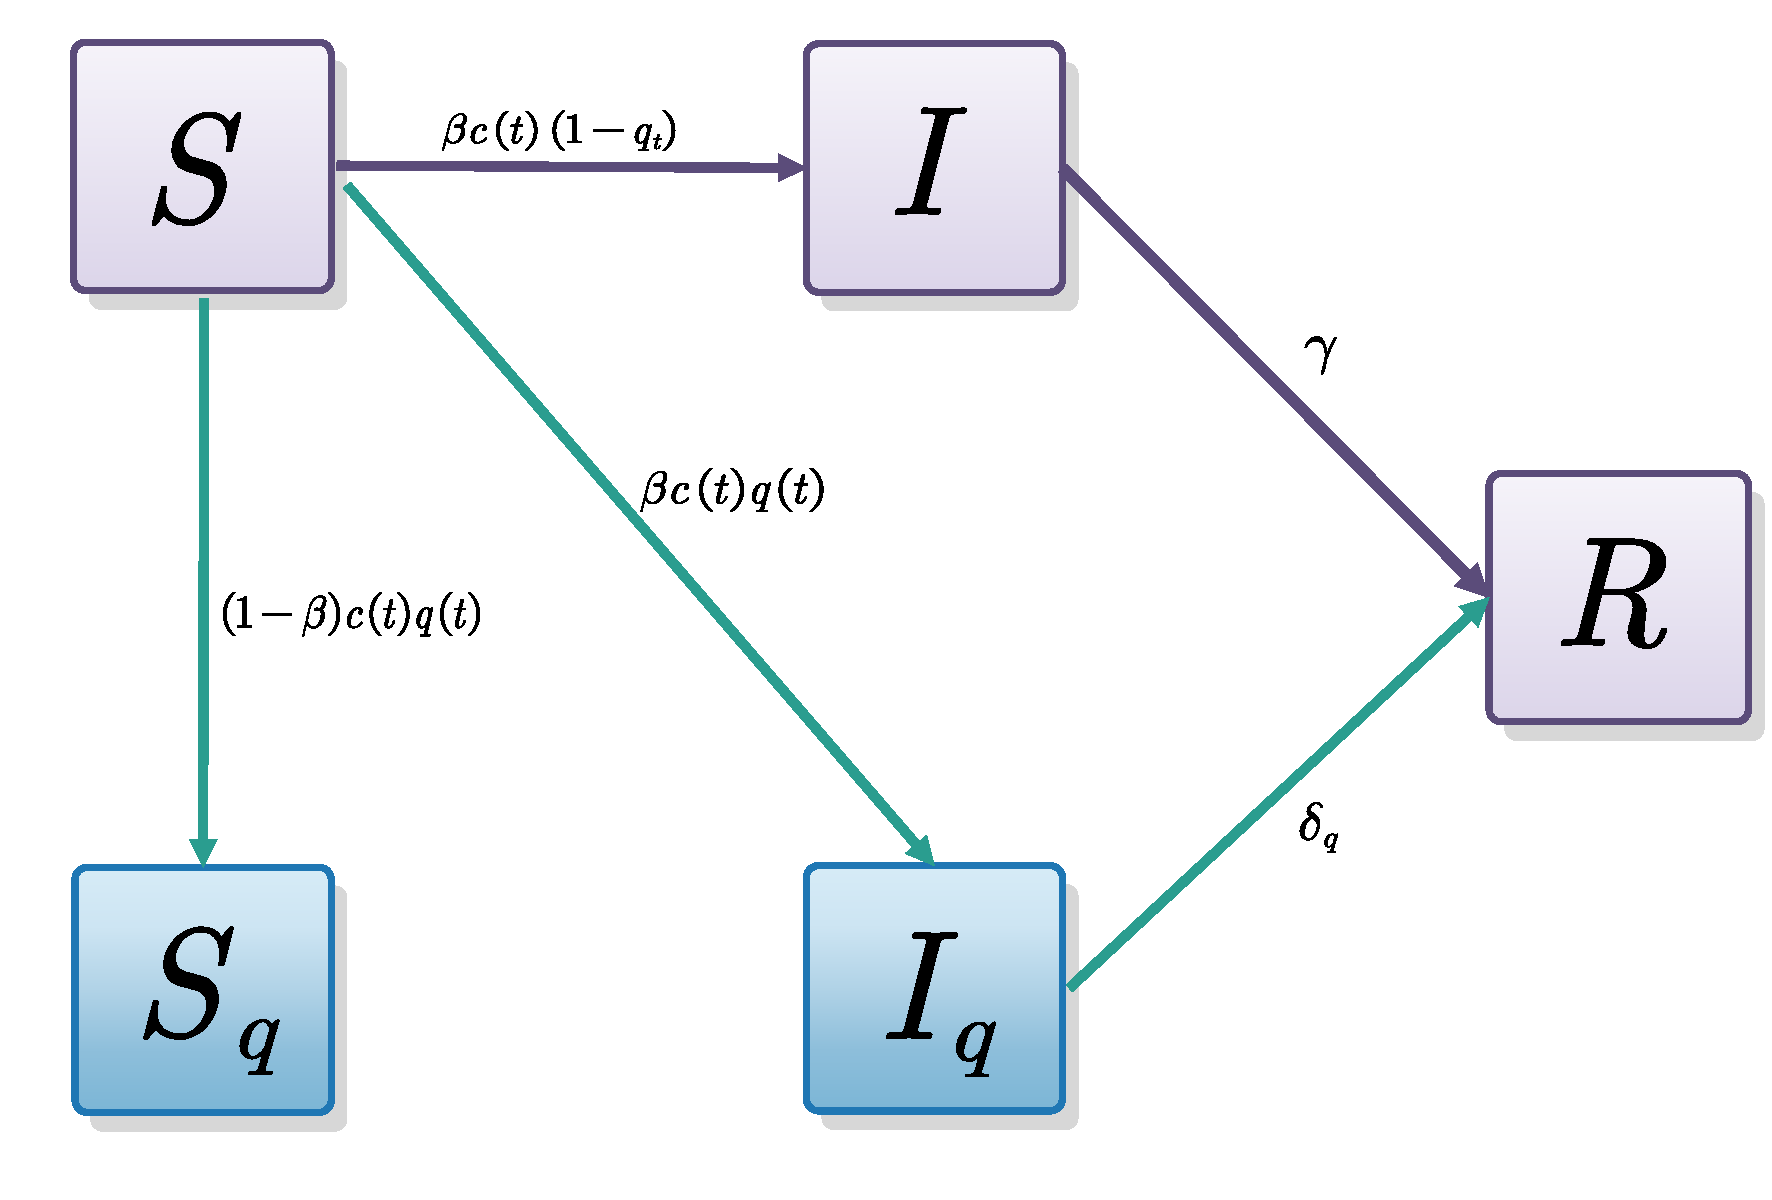
\includegraphics[width=0.7\textwidth]{figures/Fig1.pdf}
    \caption{含接触追踪与隔离的 SIQR 型模型。$S,S_q,I,I_q,R$ 分别表示社区易感者、隔离易感者、非隔离感染者、隔离感染者和康复者。}
    \label{fig:model_schematic}
\end{figure}
\subsection{医疗容量约束与三阶段控制策略}
本文以非隔离感染者人数的上限 $I(t)\le\eta$ 表示医疗容量约束，其中 $\eta$ 为给定的等效容量阈值，并不直接等同于实际 ICU 床位数。以感染人数上限表征医疗容量、并在达到上限后使感染人数维持在阈值水平的处理可见 Miclo 等的研究~\cite{Miclo2022ICU}。在本文模型中，接触率与隔离率均影响传播过程；为考察仅加强接触追踪隔离时的控制效果，固定 $c(t)\equiv c_0$，以 $q(t)$ 作为唯一的控制变量。

容量约束 $I(t)\le\eta$ 本身并不能唯一确定隔离率。本文选取一类以感染人数首次达到阈值为启动条件、以维持 $I(t)\equiv\eta$ 为控制目标的控制策略。记常规隔离率为 $0\le q_0<1$，常规接触率为 $c_0>0$，加强隔离的启动和结束时间分别为 $t_1$、$t_2$，阈值控制期隔离率记为 $q_c(t)$。控制函数为
\begin{equation}
c(t)\equiv c_0,\qquad
q(t)=
\begin{cases}
q_0, & t<t_1,\\
q_c(t), & t_1\le t\le t_2,\\
q_0, & t>t_2.
\end{cases}
\label{eq:model:piecewise-control}
\end{equation}

给定初值 $(S_0,I_0)$ 且 $0<I_0<\eta$，系统首先在常规水平 $(c_0,q_0)$ 下演化。若常规控制下的感染峰值不超过 $\eta$，则无需启动加强隔离；若该峰值超过 $\eta$，则在感染人数上升至阈值的首个时刻启动控制，即 $I(t_1)=\eta$，并记 $S^*=S(t_1)$。因此，$t_1$ 由常规传播过程和容量阈值共同确定，而不是预先指定的干预日期。

首次达到阈值时，常规控制下的感染人数仍在增加，继续采用 $q_0$ 将使 $I(t)$ 超过 $\eta$。本文假设隔离率可即时调整，在 $t_1$ 提高隔离率，并在此后的控制期内使进入非隔离感染仓室的流量与移出流量相等，即
\[
\frac{\beta c_0(1-q_c(t))}{N}S(t)=\gamma.
\]
由此在 $[t_1,t_2]$ 内维持 $I(t)\equiv\eta$，本文将这一阶段称为阈值控制期。阈值控制期内要求 $q_0\le q_c(t)\le1$。由于 $S(t)$ 仍随感染和隔离而减少，维持上述平衡所需的隔离率也随之变化，而不是一个预先给定的常数。

加强隔离的结束条件由恢复常规控制后感染人数是否继续增长决定。当 $q(t)=q_0$ 时，感染人数的增长率由 $\beta c_0(1-q_0)S/N-\gamma$ 的符号确定。因而，阈值控制期在易感者人数降至常规控制下的临界值时结束：
\begin{equation}
S(t_2)=S_c\doteq\frac{\gamma N}{\beta c_0(1-q_0)}.
\end{equation}
在本文不考虑易感者回流的模型中，恢复 $q_0$ 后 $S(t)$ 继续下降，因此 $t>t_2$ 时感染人数下降，不再超过容量阈值。相反，在阈值控制期内 $S>S_c$ 时恢复 $q_0$，感染人数会重新增加，因而不能满足所要求的上限。

本文将上述方案称为隔离率阈值控制。其启动和结束时刻分别由感染人数阈值与易感者临界值确定，控制持续时间是策略作用下的结果，而非独立指定的参数。以下研究这一给定策略的控制函数、持续时间、累计感染和成本；使感染人数维持在阈值水平是本文选定的控制要求，不作其为所有允许控制中最优方案的结论。

\subsection{常规阶段的首次积分与感染峰值}
判断阈值控制是否被触发，需要先确定常规控制下的感染峰值及其对应轨迹。式~\eqref{eq:model:full} 中，$S$ 和 $I$ 的方程不依赖于 $S_q$、$I_q$ 和 $R$，因此这一分析可归结为二维系统
\begin{equation}
\begin{cases}
\dot{S}(t) = - \beta_1(t) S(t) I(t) \\
\dot{I}(t) =   \beta_2(t) S(t) I(t) - \gamma I(t)
\end{cases}
\label{eq:model:reduced-si}
\end{equation}
其中
\begin{equation}
\beta_1(t)=\frac{c(t)\big[\beta+q(t)(1-\beta)\big]}{N},
\qquad
\beta_2(t)=\frac{\beta c(t)(1-q(t))}{N}.
\label{eq:model:beta12-general}
\end{equation}
其中 $\gamma$ 为非隔离感染者的移出率。由式~\eqref{eq:model:piecewise-control}，有
\begin{equation}
\beta_i(t)=
\begin{cases}
\beta_i^0, & t<t_1,\\
\beta_i^1(t), & t_1\le t\le t_2,\\
\beta_i^0, & t>t_2,
\end{cases}
\qquad i=1,2,
\end{equation}
其中常规防控阶段的系数为
\begin{equation}
\beta_1^0=\frac{c_0\big[\beta+q_0(1-\beta)\big]}{N},
\qquad
\beta_2^0=\frac{\beta c_0(1-q_0)}{N}.
\label{eq:model:beta12-baseline}
\end{equation}
加强隔离阶段的 $\beta_1^1(t)$ 与 $\beta_2^1(t)$ 由固定接触率 $c_0$ 和隔离控制函数 $q_c(t)$ 确定。

在前后两个常规控制阶段，$\beta_1$ 和 $\beta_2$ 均为常数，可通过消去时间变量求得首次积分。记
\begin{equation}
\rho_1=\frac{\gamma}{\beta_1^0},
\qquad
S_c=\frac{\gamma}{\beta_2^0}
=\frac{\gamma N}{\beta c_0(1-q_0)}.
\label{eq:model:baseline-symbols}
\end{equation}
其中 $S_c$ 是常规防控水平 $(c_0,q_0)$ 下的临界易感人数。给定初始状态 $(S_0,I_0)$，常规防控阶段的首次积分为
\begin{equation}
I(t)+\frac{\beta_2^0}{\beta_1^0} S(t)-\rho_1\ln S(t)
=
I_0+\frac{\beta_2^0}{\beta_1^0} S_0-\rho_1\ln S_0
\doteq C_0.
\label{eq:model:first-integral}
\end{equation}
在 $S_0>S_c$ 时，常规防控轨道上的感染人数可写为
\begin{equation*}
I(S)=I_0+\frac{\beta_2^0}{\beta_1^0}(S_0-S)
+\rho_1\ln\frac{S}{S_0}.
\end{equation*}
感染峰值在 $S=S_c$ 时取得，其值为
\begin{equation}
I_{\max}^{no}
=
I_0+\frac{\beta_2^0}{\beta_1^0}(S_0-S_c)
+\rho_1\ln\frac{S_c}{S_0}=C_0-\rho_1+\rho_1\ln S_c.
\label{eq:s1:Imax-no}
\end{equation}
将 $I_{\max}^{no}$ 与 $\eta$ 比较，即可判断常规控制是否已满足容量约束。以下主要讨论 $S_0>S_c$ 且 $0<I_0<\eta<I_{\max}^{no}$ 的情形，此时常规轨迹在达到峰值之前首次经过 $I=\eta$，加强隔离由此启动。

\section{隔离率阈值控制的解析结果}
\label{sec:s1}
常规阶段的首次积分确定了进入阈值控制期时的状态。阈值控制开始后，感染人数保持不变，但易感者人数和隔离率仍随时间变化；当系统达到退出条件后，感染人数又按常规控制下降。本节将这三个阶段连接起来，给出控制过程及其终止指标的解析表达。

按照式~\eqref{eq:model:piecewise-control}，整个过程中
\begin{equation*}
c(t)=c_0,\qquad t\ge 0,
\end{equation*}
隔离率在控制前后均为 $q_0$，阈值控制期内为 $q_c(t)$。

相应的二维系统为
\begin{equation}
\begin{cases}
\dot{S}(t) = - \beta_1(t) S(t) I(t) \\
\dot{I}(t) = \beta_2(t) S(t) I(t) - \gamma I(t)
\end{cases}
\label{eq:s1:dynamics}
\end{equation}
其中
\begin{equation}
\beta_i(t)=
\begin{cases}
\beta_i^0, & t<t_1,\\
\beta_i^1(t), & t_1\le t\le t_2,\\
\beta_i^0, & t>t_2,
\end{cases}
\quad i=1,2,
\end{equation}
其中 $\beta_1^0$ 和 $\beta_2^0$ 由式~\eqref{eq:model:beta12-baseline} 给出，阈值控制期的系数为
\begin{equation}
\beta_1^1(t)=\frac{c_0\big[\beta+q_c(t)(1-\beta)\big]}{N},
\quad
\beta_2^1(t)=\frac{\beta c_0(1-q_c(t))}{N}.
\label{eq:s1:beta12-control}
\end{equation}
记
\begin{equation}
\bar S
=
\frac{\gamma N(1-\beta)}{\beta c_0}.
\label{eq:s1:barS}
\end{equation}
由于
\[
\frac{\bar S}{S_c}
=
(1-\beta)(1-q_0)<1,
\]
故 $\bar S<S_c$。

\subsection{控制启动点与启动时间}
当 $I_0<\eta<I_{\max}^{no}$ 时，同一条常规轨迹在感染上升和下降阶段各经过一次 $I=\eta$。策略使用的是上升阶段的交点，因此求取 $S^*$ 时必须区分这两个交点。确定 $S^*$ 后，再由常规阶段的易感者方程得到启动时间。

\begin{theorem}
\label{thm:s1:trigger}
设 $S_0>S_c$ 且 $I_0<\eta<I_{\max}^{no}$。记
\begin{equation}
z_\eta:=
-\frac{1}{S_c}
\exp\left[-\frac{C_0-\eta}{\rho_1}\right] \quad z_\eta\in\left(-\frac{1}{e},0\right)
\label{eq:s1:lambert-argument}
\end{equation}
则常规控制下感染人数首次达到 $\eta$ 时，对应的易感者人数为
\begin{equation}
S^*=-S_cW_{-1}(z_\eta),
\qquad
S_c<S^*<S_0.
\label{eq:s1:Sstar-lambert}
\end{equation}
该启动状态唯一，相应的启动时间 $t_1>0$ 满足
\begin{equation}
t_1
=
\int_{S_0}^{S^*}
\frac{1}{
-\beta_1^0S\left[
C_0-\frac{\beta_2^0}{\beta_1^0}S+\rho_1\ln S
\right]
}\,dS.
\label{eq:s1:t1}
\end{equation}
\end{theorem}
\begin{proof}
加强控制启动前，系统满足首次积分~\eqref{eq:model:first-integral}。将 $I(t_1)=\eta$ 和 $S^*=S(t_1)$ 代入，得
\[
\frac{\beta_2^0}{\beta_1^0}S^*-\rho_1\ln S^*
=C_0-\eta.
\]
注意到
\[
\frac{\beta_2^0}{\beta_1^0\rho_1}
=
\frac{\beta_2^0}{\gamma}
=
\frac{1}{S_c}.
\]
于是上式可化为
\[
-\frac{1}{S_c}S^*
\exp\left(-\frac{1}{S_c}S^*\right)
=
-\frac{1}{S_c}
\exp\left[-\frac{C_0-\eta}{\rho_1}\right].
\]
由式~\eqref{eq:s1:lambert-argument}，上述方程可写为
\[
-\frac{S^*}{S_c}
\exp\left(-\frac{S^*}{S_c}\right)
=z_\eta.
\]
由 $I_{\max}^{no}=C_0-\rho_1+\rho_1\ln S_c$，可得 $z_{\eta}=-\frac{1}{e}\exp\left[-\frac{I_{\max}^{no}-\eta}{\rho_1}\right]$。结合 $\eta<I_{\max}^{no}$，有 $z_\eta\in(-1/e,0)$。因此，Lambert $W$ 函数存在两个实分支，且
\[
W_0(z_\eta)\in(-1,0),
\qquad
W_{-1}(z_\eta)\in(-\infty,-1).
\]
因此
\[
S^*=-S_cW_0(z_\eta)\in(0,S_c),
\]
或
\[
S^*=-S_cW_{-1}(z_\eta)>S_c.
\]
前者对应同一常规防控轨道在感染峰值后的下降阶段交点，后者对应感染上升阶段交点。
另一方面，在 $S\in(S_c,S_0)$ 上有
$\dot I=I(\beta_2^0S-\gamma)>0$。
结合 $I_0<\eta<I_{\max}^{no}$，常规防控轨道在到达峰值前恰有一次满足
$I(t)=\eta$，且该时刻满足 $S_c<S(t)<S_0$。
因此，首次达到阈值时对应的根唯一，应选择 $W_{-1}$ 分支，从而得到
式~\eqref{eq:s1:Sstar-lambert}。

确定 $S^*$ 后，可由常规阶段的易感者方程计算 $t_1$。由式~\eqref{eq:model:first-integral}，有
\[
I(S)=
C_0-\frac{\beta_2^0}{\beta_1^0}S+\rho_1\ln S,
\]
因此
\[
t_1
=
\int_{S_0}^{S^*}
\frac{1}{
-\beta_1^0S\left[
C_0-\frac{\beta_2^0}{\beta_1^0}S+\rho_1\ln S
\right]
}\,dS.
\]

\end{proof}

\begin{remark}
定理~\ref{thm:s1:trigger} 对应持续时间为正的阈值控制。若 $\eta=I_0$，则 $t_1=0$、$S^*=S_0$；若 $\eta=I_{\max}^{no}$，则 $z_\eta=-1/e$、$W_{-1}(z_\eta)=-1$、$S^*=S_c$，控制持续时间为零。若 $\eta>I_{\max}^{no}$，常规控制轨迹不会达到阈值；若 $\eta<I_0$，初始感染人数已超过阈值，不属于本文讨论的触发情形。
\end{remark}

\subsection{阈值控制期的隔离控制函数}
定理~\ref{thm:s1:trigger} 给出的启动状态满足 $S^*>S_c$。此时常规隔离率不足以阻止感染人数继续上升，必须提高 $q(t)$。恒定感染要求将这一选择具体化：进入 $I$ 的流量须恰好补偿其移出量，由此确定控制期的隔离率。

\begin{theorem}
\label{thm:s1:qc-structure}
设 $c(t)\equiv c_0$，且 $S_0>S_c$、$0<I_0<\eta<I_{\max}^{no}$。
若在阈值控制期 $t\in[t_1,t_2]$ 内要求 $I(t)\equiv\eta$，
则所需隔离率由下式唯一确定：
\begin{equation}
q(t)=q_c(S(t)),\qquad
q_c(S)=1-\frac{\gamma N}{\beta c_0S},\qquad S\in[S_c,S^*].
\label{eq:s1:q-control}
\end{equation}
结合控制前后采用的常规隔离率，完整的隔离控制函数为
\begin{equation}
q(t)=
\begin{cases}
q_0, & t<t_1,\\[0.35em]
q_c(S(t))=1-\dfrac{\gamma N}{\beta c_0S(t)}, & t_1\le t\le t_2,\\[0.7em]
q_0, & t>t_2.
\end{cases}
\label{eq:s1:q-piecewise}
\end{equation}
\end{theorem}

\begin{proof}
由恒定感染条件 $I(t)\equiv\eta$，有 $\dot I=0$。
代入系统~\eqref{eq:s1:dynamics} 的第二个方程，得
\[
\frac{\beta c_0(1-q)S}{N}\eta-\gamma\eta=0.
\]
由于 $\eta>0$，约去 $\eta$ 后解得
\[
q=1-\frac{\gamma N}{\beta c_0S}=q_c(S).
\]
该解唯一。结合三阶段控制的定义，即得式~\eqref{eq:s1:q-piecewise}。
\end{proof}

式~\eqref{eq:s1:q-control} 将所需隔离率表示为易感者人数的函数。沿阈值控制期轨迹考察这一关系，可进一步确定隔离率在启动和结束时是否连续，以及控制期内如何变化。这些性质如下。

\begin{corollaryn}
\label{cor:s1:qc-structure}
在定理~\ref{thm:s1:qc-structure} 的条件下，隔离控制函数具有以下性质：
\begin{enumerate}
\renewcommand{\labelenumi}{(\roman{enumi})}
    \item 启动时隔离率向上跳跃，即
    \[
    q(t_1^-)=q_0,\qquad
    q(t_1)=q(t_1^+)=q_{\max}
    =1-\frac{\gamma N}{\beta c_0S^*}>q_0.
    \]
    \item $q(t)$ 在 $(t_1,t_2)$ 上严格单调递减。
    \item 结束时隔离率连续，即
    \[
    q(t_2^-)=q(t_2)=q(t_2^+)=q_0.
    \]
\end{enumerate}
\end{corollaryn}

\begin{proof}
由式~\eqref{eq:s1:q-control} 和 $S_c=\gamma N/[\beta c_0(1-q_0)]$，有
\[
q_c(S_c)=q_0,\qquad q_c(S^*)=q_{\max}.
\]
在 $t=t_1$ 左侧系统仍采用常规隔离率，故 $q(t_1^-)=q_0$。
进入阈值控制期后，$q(t_1)=q(t_1^+)=q_c(S^*)=q_{\max}$，且
\[
\Delta q:=q_{\max}-q_0
=\frac{\gamma N}{\beta c_0}
\left(\frac{1}{S_c}-\frac{1}{S^*}\right)>0,
\]
其中 $S^*>S_c$，故 (i) 成立。

将 $q_c(S)$ 代入 $S$ 方程，得
\[
\dot S=-\frac{c_0\eta}{N}(S-\bar S),\qquad
\bar S=\frac{(1-\beta)\gamma N}{\beta c_0}.
\]
因此，沿阈值控制期轨迹有
\[
\frac{d}{dt}q_c(S(t))
=\frac{\gamma N}{\beta c_0}\frac{\dot S(t)}{S(t)^2}
=-\frac{\gamma\eta}{\beta}\frac{S(t)-\bar S}{S(t)^2}<0,
\qquad t_1<t<t_2,
\]
由于 $S(t)\ge S_c>\bar S$，(ii) 成立。

由 $S(t_2)=S_c$，得 $q(t_2^-)=q(t_2)=q_c(S_c)=q_0$。
而 $t>t_2$ 时隔离率恢复为 $q_0$，因此 $q(t_2^+)=q_0$，(iii) 成立。
\end{proof}

\begin{remark}
式~\eqref{eq:s1:q-control} 给出隔离控制函数的状态表达。代入下一小节的理论轨迹后，可得时间函数 $q_c(t)$；本文数值计算采用该预定函数，不作实时反馈修正。
\end{remark}

\subsection{阈值控制期的状态轨迹与控制持续时间}
上述隔离控制函数给出了隔离率与状态的关系，但确定其时间变化和持续时间还需要求出 $S(t)$。代入恒定感染条件后，易感者方程化为 $\dot S=-(c_0\eta/N)(S-\bar S)$，因此阈值控制期轨迹可以显式求得，并据此将隔离控制函数写为时间的函数。
\begin{theorem}
    在定理~\ref{thm:s1:qc-structure} 的条件下，阈值控制期 $t\in[t_1,t_2]$ 内的易感者人数为
    \begin{equation}
        S(t) = \left( S^* - \bar S \right) e^{\frac{-c_0\eta}{N}(t - t_1 )} + \bar S
        \label{eq:s1:S-analytic}
    \end{equation}
    隔离控制函数为
    \begin{equation*}
    q(t) =
    \begin{cases}
    q_0, & t < t_1, \\
    q_c(t) & t_1 \le t \le t_2, \\
    q_0, & t > t_2.       
    \end{cases}
    \end{equation*}
    其中
    \begin{equation}
        q_c(t)= 1 - \frac{1}{\left[\frac{\beta c_0 S^* }{\gamma N} + \beta- 1 \right] e^{\frac{-c_0 \eta}{N} (t-t_1)} + 1-\beta} 
    \end{equation}
\end{theorem}
\begin{proof}
    求解一阶线性方程 $\dot{S}=-\frac{c_0\eta}{N}(S-\bar S)$，得
    \[
        S(t) = C e^{\frac{-c_0 \eta}{N} t} + \bar S
    \]
    其中 $C$ 为积分常数。代入初值 $S(t_1)=S^*$，得
    \[
    S(t) = \left( S^* - \bar S \right) e^{\frac{-c_0\eta}{N}(t - t_1 )} + \bar S
    \]
    将 $S(t)$ 代入 $q_c(S(t))=1-\frac{\gamma N}{\beta c_0 S(t)}$，得到关于时间的控制函数：
    \[
    q_c(t)= 1 - \frac{1}{\left[\frac{\beta c_0 S^* }{\gamma N} + \beta- 1 \right] e^{\frac{-c_0 \eta}{N} (t-t_1)} + 1-\beta}
    \]
\end{proof}
式~\eqref{eq:s1:S-analytic} 描述了阈值控制期内易感者人数的下降过程。加强隔离并不在预定日期结束，而是持续到 $S(t)$ 达到 $S_c$。由于 $S^*>S_c>\bar S$，该轨迹在有限时间内达到退出状态，所需时间由下面的结果给出。

\begin{theorem}
    在定理~\ref{thm:s1:qc-structure} 的条件下，以 $S(t_2)=S_c$ 为结束条件，则控制结束时间为
    \begin{equation}
    t_2
    =
    t_1+
    \frac{N}{c_0 \eta}
    \ln \left[
    \frac{S^*-\bar S}
    {S_c-\bar S}
    \right]
    \label{eq:s1:t2}
    \end{equation}
    相应的控制持续时间为
        \begin{equation}
        \Delta t = \frac{N}{c_0 \eta}
        \ln \left[
        \frac{S^*-\bar S}
        {S_c-\bar S}
        \right]
    \end{equation}
\end{theorem}
\begin{proof}   
    阈值控制期内，易感者人数从 $S^*$ 下降至 $S_c$。对易感者方程积分，得
    \begin{align*}
        \Delta t=t_2-t_1=\int_{t_1}^{t_2} dt=&\int_{S^*}^{S_c} \frac{1}{\dot{S}} \, dS
        =\frac{N}{c_0\eta}\int_{S_c}^{S^*} \frac{1}{S-\bar S}\,dS
        =\frac{N}{c_0 \eta}
        \ln \left[
        \frac{S^*-\bar S}
        {S_c-\bar S}
        \right].
    \end{align*}
    因此，
    \begin{equation*}
    t_2
    =
    t_1+
    \frac{N}{c_0 \eta}
    \ln \left[
    \frac{S^*-\bar S}
    {S_c-\bar S}
    \right]=\int_{S_0}^{S^*}
    \frac{1}{
    -\beta_1^0S\left[
    C_0-\frac{\beta_2^0}{\beta_1^0}S+\rho_1\ln S
    \right]
    }\,dS + \frac{N}{c_0 \eta}
    \ln \left[
    \frac{\frac{\beta c_0}{\gamma N}S^*+ \beta-1}
    {\frac{q_0}{1-q_0}+ \beta}
    \right]
    \end{equation*}
\end{proof}

\begin{remark}
    将结束条件 $S(t_2)=S_c=\frac{\gamma N}{\beta c_0(1-q_0)}$ 代入式~\eqref{eq:s1:S-analytic}，亦得
    \begin{equation*}
     t_2= t_1+\frac{N}{c_0 \eta}
     \ln \left[
     \frac{S^*-\bar S}
     {S_c-\bar S}
     \right]
    \end{equation*}
    以及控制持续时间
    \begin{equation*}
    \Delta t = \frac{N}{c_0 \eta}
     \ln \left[
     \frac{S^*-\bar S}
     {S_c-\bar S}
     \right]
    \end{equation*}
\end{remark}
\begin{remark}
    在 $S(t)=C e^{\frac{-c_0 \eta}{N}t}+\bar S$ 中代入结束条件 $S(t_2)=S_c$，可写为
    \begin{equation*}
    S(t) = \left( S_c - \bar S \right) e^{\frac{c_0\eta}{N}(t_2 - t )} + \bar S
    \end{equation*}
    再代入 $q_c(S(t))=1-\frac{\gamma N}{\beta c_0S(t)}$，隔离控制函数可写为
    \begin{align*}
    q_c(t)=1 - \frac{1}{(\tfrac{q_0}{1-q_0}+\beta)e^{\frac{c_0\eta}{N}(t_2 - t )}+1-\beta}
    \end{align*}
\end{remark}

\subsection{动态清零时间}
控制结束并不等于感染过程结束：在 $t_2$ 时仍有 $I(t_2)=\eta$。恢复常规隔离率后，$S(t)<S_c$，感染人数随之下降；当 $\eta>1$ 时，还需要一段时间才能达到社区动态清零。因此，控制持续时间与疫情持续时间应分别计算。

沿用 Zhou 等~\cite{Zhou2024SPCI} 对隔离区外动态清零的定义，本文以非隔离感染者人数在下降阶段达到 $1$ 作为判据，记相应时刻为 $t_{end}$，即 $I(t_{end})=1$ 且 $I'(t_{end})<0$。退出后的常规轨迹从 $(S_c,\eta)$ 出发，利用同一首次积分即可确定该时刻及其对应的易感者人数。
\begin{theorem}\label{thm:s1:tend}
    在上述阈值控制下，设动态清零时刻位于控制结束之后。记 $C_2=\eta+(\beta_2^0/\beta_1^0)S_c-\rho_1\ln S_c$，则 $t_{end}$ 由下式给出
    \[
    t_{end}=t_2+\int_{S_c}^{S(t_{end})}\frac{1}
    {S\left[\beta_2^0 S-\beta_1^0 \rho_1 \ln(S)-
    \beta_1^0 C_2\right]}\, dS .
    \]
    其中
    \begin{equation}
    S(t_{end})=
    -\frac{\beta_1^0 \rho_1}{\beta_2^0}\,
    \operatorname{LambertW}_0
    \left(
    -\frac{\beta_2^0}{\beta_1^0 \rho_1}
    \exp\left(
    \frac{1-C_2}{\rho_1}
    \right)
    \right).
    \label{eq:s1:Send}
    \end{equation}
\end{theorem}
\begin{proof}
    由于在阈值控制中，当 $t\ge t_2$ 时，系统恢复到常规防控水平
    \[
    c(t)=c_0,\qquad q(t)=q_0.
    \]
    因此，$t\in[t_2,+\infty)$ 上仍满足常规阶段的首次积分。不过此时首次积分常数由
    $t=t_2$ 时刻的状态决定。记
    \[
    C_2=\eta+\frac{\beta_2^0}{\beta_1^0}S(t_2)-\rho_1\ln S(t_2)=\eta+\frac{\beta_2^0}{\beta_1^0}S_c-\rho_1\ln S_c.
    \]
    于是
    \[
    I(t)
    =
    -\frac{\beta_2^0}{\beta_1^0} S(t)
    +
    \rho_1 \ln S(t)
    +
    C_2,
    \qquad
    t \in [t_2,+\infty).
    \]
    由 $I(t_{end})=1$ 和 $I'(t_{end})<0$ 得到
    \[
    1
    +
    \frac{\beta_2^0}{\beta_1^0} S(t_{end})
    -
    \rho_1 \ln(S(t_{end}))
    =
    C_2 .
    \]
    同时满足 $S(t_{end})<\frac{\gamma}{\beta_2^0}$。利用 Lambert $W$ 函数求解，得到
    \[
    S(t_{end})=
    -\frac{\beta_1^0 \rho_1}{\beta_2^0}\,
    \operatorname{LambertW}_0
    \left(
    -\frac{\beta_2^0}{\beta_1^0 \rho_1}
    \exp\left(
    \frac{1-C_2}{\rho_1}
    \right)
    \right).
    \]
    于是
    \[
    S'(t)=S\left[\beta_2^0 S-
    \beta_1^0 \rho_1 \ln(S)
    -\beta_1^0 C_2
    \right],
    \qquad
    t \in [t_2,+\infty).
    \]
    从时间 $t_2$ 积分到 $t_{end}$，有
    \[
    \int_{S_c}^{S(t_{end})}
    \frac{1}
    {
    S\left[
    \beta_2^0 S
    -
    \beta_1^0 \rho_1 \ln(S)
    -
    \beta_1^0 C_2
    \right]
    }
    \, dS
    =
    \int_{t_2}^{t_{end}} dt .
    \]

    因此
    \[
    t_{end}=t_2+\int_{S_c}^{S(t_{end})}\frac{1}
    {S\left[\beta_2^0 S-\beta_1^0 \rho_1 \ln(S)-
    \beta_1^0 C_2\right]}\, dS .
    \]
\end{proof}


\subsection{总累计感染}
峰值约束只限制同时存在的非隔离感染者人数，不能由此确定整个过程的累计感染规模。阈值控制期虽有 $I(t)\equiv\eta$，仍不断出现新感染者；此外，直接进入 $I_q$ 的感染者也应计入总数。为与动态清零时间采用同一评价终点，将从初始时刻到动态清零时刻的总累计感染定义为
\begin{equation}
\Itcum
=
\int_0^{t_{\rm end}}\frac{\beta c(t)}{N}S(t)I(t)\,dt.
\end{equation}
同时，进入社区感染仓室 $I$ 与进入隔离感染仓室 $I_q$ 的累计感染分别为
\begin{equation}
I_{\rm cum}
=
\int_0^{t_{\rm end}}
\frac{\beta c(t)(1-q(t))}{N}S(t)I(t)\,dt,
\end{equation}
和
\begin{equation}
I_{q_{\rm cum}}
=
\int_0^{t_{\rm end}}
\frac{\beta c(t)q(t)}{N}S(t)I(t)\,dt.
\end{equation}
于是
\[
\Itcum=I_{\rm cum}+I_{q_{\rm cum}}.
\]

前后两个常规阶段具有相同的参数，感染流量均可用易感者人数的变化表示；阈值控制阶段则使用已求得的 $S(t)$ 和 $q_c(t)$。分别计算三段流量，可将累计感染写成启动、退出和清零时刻的易感者人数的函数。

\begin{theorem}\label{thm:s1:Itcum}
    设系统在 $t_1$ 启动阈值控制，在 $t_2$ 结束控制，并在 $t_{\rm end}>t_2$ 达到动态清零。记 $S_{\rm end}=S(t_{\rm end})$，则从初始时刻到 $t_{\rm end}$ 的总累计感染为
    \[
    \Itcum
    =
    \frac{\beta}{\beta+q_0(1-\beta)}(S_0-S^*)
    +
    \beta\left[
    (S^*-S_c)+\bar S\ln\frac{S^*-\bar S}{S_c-\bar S}
    \right]
    +
    \frac{\beta}{\beta+q_0(1-\beta)}(S_c-S_{\rm end}).
    \]
\end{theorem}
\begin{proof}
    记总新发感染率为
    \[
    F(t)=\frac{\beta c(t)}{N}S(t)I(t).
    \]
    在第一段常规阶段 $0\le t\le t_1$，有 $c(t)=c_0,\ q(t)=q_0$，故
    \[
    \dot S
    =
    -\frac{c_0[\beta+q_0(1-\beta)]}{N}SI.
    \]
    因而
    \[
    F(t)
    =
    \frac{\beta}{\beta+q_0(1-\beta)}(-\dot S).
    \]
    从 $0$ 到 $t_1$ 积分，并利用 $S(t_1)=S^*$，得到
    \[
    \int_0^{t_1}F(t)\,dt
    =
    \frac{\beta}{\beta+q_0(1-\beta)}(S_0-S^*).
    \]

    在阈值控制阶段 $t_1\le t\le t_2$，有 $I(t)\equiv\eta$，且
    \[
    q_c(t)=1-\frac{\gamma N}{\beta c_0S(t)}.
    \]
    由 $S$ 方程可得
    \[
    \dot S
    =
    -\frac{c_0\eta}{N}(S-\bar S),
    \qquad
    \bar S=\frac{(1-\beta)\gamma N}{\beta c_0}.
    \]
    因此
    \[
    dt
    =
    -\frac{N}{c_0\eta}\frac{dS}{S-\bar S}.
    \]
    又因为此时
    \[
    F(t)=\frac{\beta c_0}{N}S(t)\eta,
    \]
    所以
    \[
    \int_{t_1}^{t_2}F(t)\,dt
    =
    \beta\int_{S_c}^{S^*}\frac{S}{S-\bar S}\,dS
    =
    \beta\left[
    (S^*-S_c)+\bar S\ln\frac{S^*-\bar S}{S_c-\bar S}
    \right].
    \]

    在解除控制后的常规阶段 $t_2\le t\le t_{\rm end}$，仍有
    $c(t)=c_0,\ q(t)=q_0$，因此与第一段相同，
    \[
    F(t)
    =
    \frac{\beta}{\beta+q_0(1-\beta)}(-\dot S).
    \]
    由 $S(t_2)=S_c$ 与 $S(t_{\rm end})=S_{\rm end}$ 得
    \[
    \int_{t_2}^{t_{\rm end}}F(t)\,dt
    =
    \frac{\beta}{\beta+q_0(1-\beta)}(S_c-S_{\rm end}).
    \]

    三段相加即得结论。
\end{proof}

\section{成本与参数敏感性}
\label{sec:cost}
第~\ref{sec:s1}~节确定了给定参数下的三阶段控制过程。不同容量阈值和常规接触水平会改变启动状态、所需隔离率及控制持续时间，因而即使都能满足各自的感染上限，控制投入也可能不同。本节以累计控制强度评价这一投入，并分析有关指标的参数依赖。

以下分析均在相应结论规定的参数范围内进行。对某一参数求偏导时，除特别说明外，固定人口规模、初始状态及其余独立参数。

\subsection{成本函数}

为与其他控制方案采用统一指标进行比较，本文保留接触率和隔离率两个分项归一化成本
\begin{equation}
J_c=\int_{t_1}^{t_2} \frac{\bigl(c_0-c(t)\bigr)_+}{c_0}\,dt,
\end{equation}
\begin{equation}
J_q=\int_{t_1}^{t_2} \frac{\bigl(q(t)-q_0\bigr)_+}{1-q_0}\,dt.
\end{equation}
其中 $(x)_+=\max\{x,0\}$。进一步定义二次加权综合成本
\begin{equation}
J
=
\int_{t_1}^{t_2}
\left[
\left(\frac{\bigl(c_0-c(t)\bigr)_+}{c_0}\right)^2
+
2\left(\frac{\bigl(q(t)-q_0\bigr)_+}{1-q_0}\right)^2
\right]dt.
\label{eq:cost:J}
\end{equation}
式~\eqref{eq:cost:J} 的被积函数为归一化控制强度，不显含人口规模 $N$。

隔离项的权重取为 $2$，表示在该成本设定下加强隔离的单位强度成本较高。本文阈值策略保持 $c(t)\equiv c_0$，故 $J_c=0$，额外成本仅来自隔离率的提高。
利用控制期内
\[
\dot S=-\frac{c_0\eta}{N}(S-\bar S),
\]
可将阈值控制中的 $J_q$ 写为
\begin{equation}
J_q
=
\frac{N}{\eta(1-q_0)}
\int_{S_c}^{S^*}
\frac{q_c(S)-q_0}{c_0(S-\bar S)}\,dS.
\end{equation}
当 $\eta$ 增大时，上限 $S^*$ 下降，同时前面的 $1/\eta$ 下降，故额外累计控制强度随
$\eta$ 增大而下降。对于 $c_0$，积分上限、终点阈值、被积函数以及时间尺度同时改变，
这些变化的作用方向不同，需结合后续数值结果判断。


\subsection{启动点的参数敏感性}
控制持续时间、最大隔离率和成本的表达式都含有 $S^*$，而 $S^*$ 又由常规轨迹与感染阈值的交点确定。因此，分析这些指标时需要同时计入启动状态的变化，不能把 $S^*$ 视为独立于参数的常量。下面先给出其参数导数的符号，作为后续分析的依据。

\begin{lemma}
\label{lem:s1:Sstar-sensitivity}
设 $S_0>S_c$ 且 $I_0<\eta<I_{\max}^{no}$。固定其余参数时，
启动点 $S^*$ 满足
\[
\frac{\partial S^*}{\partial \eta}<0,
\qquad
\frac{\partial S^*}{\partial c_0}>0,
\qquad
\frac{\partial S^*}{\partial \beta}>0,
\qquad
\frac{\partial S^*}{\partial q_0}<0.
\]
若固定 $N,S_0,I_0$ 并以 $\theta=\eta/N$ 为参数，则
\[
\frac{\partial S^*}{\partial \theta}=N\frac{\partial S^*}{\partial \eta}<0.
\]
\end{lemma}

\begin{proof}
由常规控制阶段的首次积分，启动点满足
\begin{equation}
\begin{aligned}
F(S^*;\eta,c_0,\beta,q_0)
:={}&
I_0+
\frac{\beta(1-q_0)}
{\beta+q_0(1-\beta)}
(S_0-S^*) \\
&+
\rho_1\ln\frac{S^*}{S_0}
-\eta
=0.
\end{aligned}
\label{eq:s1:F-Sstar-param}
\end{equation}
由于 $\rho_1/S_c=\beta(1-q_0)/[\beta+q_0(1-\beta)]$，
\[
\frac{\partial F}{\partial S^*}
=
\rho_1
\left(
\frac1{S^*}-\frac1{S_c}
\right)<0,
\]
由于启动时感染人数处于上升阶段，有 $S^*>S_c$，故上述偏导数非零，隐函数定理适用。

首先，$\frac{\partial F}{\partial \eta}=-1$，故
\begin{equation}
\frac{\partial S^*}{\partial \eta}
=
\frac{1}{
\rho_1
\left(
\dfrac1{S^*}-\dfrac1{S_c}
\right)
}
<0.
\label{eq:s1:Sstar-eta-sign}
\end{equation}
其次，$\frac{\partial \rho_1}{\partial c_0}=-\rho_1/c_0$，从而
\[
\frac{\partial F}{\partial c_0}
=
-\frac{\rho_1}{c_0}\ln\frac{S^*}{S_0}>0,
\]
并有
\begin{equation}
\frac{\partial S^*}{\partial c_0}
=
\frac{\ln(S^*/S_0)}
{c_0
\left(
\dfrac1{S^*}-\dfrac1{S_c}
\right)
}
>0.
\label{eq:s1:Sstar-c0-sign}
\end{equation}

对 $\beta$，固定 $S^*$ 时
\[
\frac{\partial}{\partial\beta}
\frac{\beta(1-q_0)}
{\beta+q_0(1-\beta)}
=
\frac{q_0(1-q_0)}
{\left[\beta+q_0(1-\beta)\right]^2},
\]
\[
\frac{\partial \rho_1}{\partial \beta}
=
-\frac{\rho_1(1-q_0)}
{\beta+q_0(1-\beta)}.
\]
因此
\begin{equation}
\frac{\partial S^*}{\partial \beta}
=
\frac{
\displaystyle
\frac{q_0(1-q_0)}
{\left[\beta+q_0(1-\beta)\right]^2}
(S_0-S^*)
-
\frac{\rho_1(1-q_0)}
{\beta+q_0(1-\beta)}
\ln\frac{S^*}{S_0}
}{
\displaystyle
\rho_1
\left(
\frac1{S_c}-\frac1{S^*}
\right)
}
>0.
\label{eq:s1:Sstar-beta-sign}
\end{equation}
上式分母为正。由 $S_0>S^*$、$\ln(S^*/S_0)<0$，分子第一项非负、第二项严格为正，故 $\frac{\partial S^*}{\partial \beta}>0$。

最后，对 $q_0$ 有
\[
\frac{\partial}{\partial q_0}
\frac{\beta(1-q_0)}
{\beta+q_0(1-\beta)}
=
-\frac{\beta}
{\left[\beta+q_0(1-\beta)\right]^2},
\qquad
\frac{\partial \rho_1}{\partial q_0}
=
-\frac{\rho_1(1-\beta)}
{\beta+q_0(1-\beta)}.
\]
利用
\[
\frac{\rho_1(1-\beta)}
{\beta+q_0(1-\beta)}
=
\frac{\beta\bar S}
{\left[\beta+q_0(1-\beta)\right]^2},
\]
可得
\begin{equation}
\frac{\partial S^*}{\partial q_0}
=
-\frac{
\beta
\left[
(S_0-S^*)
-\bar S\ln\frac{S_0}{S^*}
\right]
}{
\left[\beta+q_0(1-\beta)\right]^2
\rho_1
\left(
\dfrac1{S_c}-\dfrac1{S^*}
\right)
}
<0.
\label{eq:s1:Sstar-q0-sign}
\end{equation}
事实上，由 $\bar S<S^*<S_0$ 及 $\ln x<x-1$（$x>1$）知
\[
\bar S\ln\frac{S_0}{S^*}
<
S^*\ln\frac{S_0}{S^*}
<
S_0-S^*,
\]
故式~\eqref{eq:s1:Sstar-q0-sign} 方括号内严格为正。
当固定 $N$ 且 $\eta=N\theta$ 时，链式法则给出
$\frac{\partial S^*}{\partial \theta}=N\frac{\partial S^*}{\partial \eta}<0$。
\end{proof}

\subsection{启动时间与最大隔离率的参数敏感性}
启动点的变化反映加强隔离时的易感者规模，启动时间还取决于到达该状态的速度；两者的变化方向不能直接等同。最大隔离率则由启动状态和传播参数共同决定。以下分别考察常规接触率与医疗容量阈值
\[
c_0,\qquad \eta .
\]
的影响，固定其余参数，并限定在常规轨迹于感染上升阶段达到阈值的范围内。

为便于书写，记
\begin{equation}
a=\frac{\beta_2^0}{\beta_1^0}
=
\frac{\beta(1-q_0)}{\beta+q_0(1-\beta)},
\qquad
\rho_1=\frac{\gamma}{\beta_1^0}
=
\frac{\gamma N}{c_0[\beta+q_0(1-\beta)]},
\end{equation}
以及
\begin{equation}
S_c=\frac{\gamma}{\beta_2^0}
=
\frac{\gamma N}{\beta c_0(1-q_0)}.
\end{equation}
注意到 $a$ 与 $c_0$ 无关，而 $\rho_1$ 与 $S_c$ 均与 $c_0$ 成反比。

改变 $c_0$ 还可能使常规感染峰值降至阈值以下，此时加强隔离不再被触发。因此，在比较启动时间和隔离强度之前，先确定阈值控制被触发的参数范围。固定 $\eta$ 及 $N,S_0,I_0,\beta,\gamma,q_0$，记常规控制下的感染峰值为 $I_{\max}^{no}(c_0)$，定义临界接触率
\begin{equation}
c_{0,\min}(\eta)
=
\inf\left\{
c_0>0:
I_{\max}^{no}(c_0)\geq \eta
\right\}.
\label{eq:s1:c0-min-def}
\end{equation}
由式~\eqref{eq:s1:Imax-no}，并利用
$\beta_2^0/\beta_1^0=a$、$\rho_1=aS_c$，可将常规控制下的峰值写为
\begin{equation}
I_{\max}^{no}(c_0)
=
I_0+a(S_0-S_c)+aS_c\ln\frac{S_c}{S_0}.
\label{eq:s1:Imax-no-c0}
\end{equation}
当 $S_0>S_c$、感染人数在初始阶段增加时，
\begin{equation}
\frac{d I_{\max}^{no}}{dc_0}
=
-\frac{aS_c}{c_0}\ln\frac{S_c}{S_0}>0.
\label{eq:s1:Imax-no-c0-derivative}
\end{equation}
若给定阈值满足
$I_0<\eta<I_0+aS_0$，式~\eqref{eq:s1:c0-min-def} 所定义的临界值在上述参数范围内存在且唯一，并满足
\begin{equation}
I_{\max}^{no}\!\left(c_{0,\min}(\eta)\right)=\eta.
\label{eq:s1:c0-min-equality}
\end{equation}
后文固定 $\eta$ 时，将 $c_{0,\min}(\eta)$ 简记为 $c_{0,\min}$。于是
\begin{equation}
\begin{aligned}
c_0<c_{0,\min}
&\quad\Longrightarrow\quad I_{\max}^{no}(c_0)<\eta,\\
c_0=c_{0,\min}
&\quad\Longrightarrow\quad I_{\max}^{no}(c_0)=\eta,\\
c_0>c_{0,\min}
&\quad\Longrightarrow\quad I_{\max}^{no}(c_0)>\eta.
\end{aligned}
\label{eq:s1:c0-min-regimes}
\end{equation}
当 $c_0<c_{0,\min}$ 时，无需加强隔离；当 $c_0=c_{0,\min}$ 时，轨迹在感染峰值处与 $I=\eta$ 相切，$S^*=S_c$ 且 $\Delta t=0$；当 $c_0>c_{0,\min}$ 时，控制持续时间为正。
相应地，
\begin{equation}
c_0\downarrow c_{0,\min}^{+}
\quad\Longrightarrow\quad
S^*\to S_c,
\qquad
\Delta t\to0.
\label{eq:s1:c0-min-limit}
\end{equation}
在 $c_0>c_{0,\min}$ 时，$\Delta t$ 的变化方向由推论~\ref{cor:s1:duration-sensitivity} 给出的导数判据确定。

\begin{proposition}
\label{prop:s1:sensitivity}
设参数满足以下触发条件：
\[
c_0>c_{0,\min}(\eta),
\qquad
I_0<\eta<I_{\max}^{no}(c_0),
\qquad
S_0>S^*>S_c>\bar S.
\]
固定其余参数，启动时间和最大隔离率满足
\[
\frac{\partial t_1}{\partial \eta}>0,
\qquad
\frac{\partial t_1}{\partial c_0}<0,
\]
以及
\[
\frac{\partial q_{\max}}{\partial \eta}<0,
\qquad
\frac{\partial q_{\max}}{\partial c_0}>0.
\]
\end{proposition}

\begin{proof}
由引理~\ref{lem:s1:Sstar-sensitivity}，有
$\frac{\partial S^*}{\partial \eta}<0$ 与 $\frac{\partial S^*}{\partial c_0}>0$。启动时间可写为
\begin{equation}
t_1
=
\frac{N}{c_0\bigl[\beta+q_0(1-\beta)\bigr]}
\int_{S^*}^{S_0}
\frac{1}{S I(S;c_0)}\,dS,
\qquad
I(S;c_0)
=
I_0-a(S-S_0)+\rho_1\ln\frac{S}{S_0}.
\end{equation}
由于积分下端满足 $I(S^*;c_0)=\eta$，对 $\eta$ 求导得到
\begin{equation}
\frac{\partial t_1}{\partial \eta}
=
-\frac{N}{c_0\bigl[\beta+q_0(1-\beta)\bigr]}
\frac{1}{S^*\eta}
\frac{\partial S^*}{\partial \eta}>0.
\end{equation}
对 $c_0$ 求导，有
\[
\frac{\partial I(S;c_0)}{\partial c_0}
=
-\frac{\rho_1}{c_0}\ln\frac{S}{S_0}>0,
\qquad S\in(S^*,S_0),
\]
从而
\begin{align}
\frac{\partial t_1}{\partial c_0}
=&
-\frac{N}{c_0^2\bigl[\beta+q_0(1-\beta)\bigr]}
\int_{S^*}^{S_0}\frac{1}{S I(S;c_0)}\,dS
-\frac{N}{c_0\bigl[\beta+q_0(1-\beta)\bigr]}
\frac{1}{S^*\eta}
\frac{\partial S^*}{\partial c_0} \nonumber\\
&-\frac{N}{c_0\bigl[\beta+q_0(1-\beta)\bigr]}
\int_{S^*}^{S_0}
\frac{\frac{\partial I(S;c_0)}{\partial c_0}}{S I^2(S;c_0)}\,dS
<0.
\end{align}


由隔离控制函数的表达式
\[
q_c(S)=1-\frac{\gamma N}{\beta c_0S},
\qquad
\frac{dq_c}{dS}
=
\frac{\gamma N}{\beta c_0S^2}>0.
\]
控制期内 $S(t)$ 单调下降，因此 $q_c(t)$ 在控制期内单调下降，最大值出现在启动时刻 $t_1$：
\[
q_{\max}
=
q_c(t_1)
=
1-\frac{\gamma N}{\beta c_0S^*}.
\]
于是
\[
\frac{\partial q_{\max}}{\partial \eta}
=
\frac{\gamma N}{\beta c_0(S^*)^2}\frac{\partial S^*}{\partial \eta}<0,
\]
以及
\[
\frac{\partial q_{\max}}{\partial c_0}
=
\frac{\gamma N}{\beta c_0^2(S^*)^2}
\left(S^*+c_0\frac{\partial S^*}{\partial c_0}\right)>0.
\]
\end{proof}

\subsection{控制时长的参数敏感性}
命题~\ref{prop:s1:sensitivity} 表明，增大 $c_0$ 会使控制更早启动，并提高启动时所需的隔离率，但这并不直接决定阈值控制需持续多久。式~\eqref{eq:s1:t2} 中，参数既改变起止状态，也改变时间尺度，控制时长的导数需要同时考虑这些作用。结合启动点的参数导数，可得以下结果。

\begin{corollaryn}
\label{cor:s1:duration-sensitivity}
设 $S_0>S_c$ 且 $I_0<\eta<I_{\max}^{no}$。固定其余参数时，有
\[
\frac{\partial \Delta t}{\partial \eta}<0,
\qquad
\frac{\partial \Delta t}{\partial \beta}>0,
\qquad
\frac{\partial \Delta t}{\partial q_0}<0.
\]
若固定 $N,S_0,I_0$，则
$\frac{\partial \Delta t}{\partial \theta}=N\frac{\partial \Delta t}{\partial \eta}<0$。
另一方面，$\frac{\partial \Delta t}{\partial c_0}$ 没有固定符号。令
\[
\Theta
=
\frac{S^*-S_c}{S_c}
\left[
\frac{S^*-\bar S}{S^*}
\ln\frac{S^*-\bar S}{S_c-\bar S}
-1
\right],
\]
则
\[
\frac{\partial\Delta t}{\partial c_0}
\gtrless0
\quad\Longleftrightarrow\quad
\ln\frac{S_0}{S^*}
\gtrless\Theta,
\]
等号情形亦对应成立。特别地，若 $\Theta\le0$，则
$\partial\Delta t/\partial c_0>0$。
\end{corollaryn}

\begin{proof}
由
\[
\Delta t
=
\frac{N}{c_0\eta}
\ln\frac{S^*-\bar S}{S_c-\bar S}
\]
及 $\frac{\partial S^*}{\partial \eta}<0$，有
\[
\frac{\partial\Delta t}{\partial\eta}
=
-\frac{N}{c_0\eta^2}
\ln\frac{S^*-\bar S}{S_c-\bar S}
+
\frac{N}{c_0\eta}
\frac{\frac{\partial S^*}{\partial \eta}}{S^*-\bar S}
<0.
\]
固定 $N$ 时 $\eta=N\theta$，故
$\frac{\partial \Delta t}{\partial \theta}=N\frac{\partial \Delta t}{\partial \eta}<0$；等价地，
\[
\frac{\partial\Delta t}{\partial\theta}
=
\frac1{c_0}
\left[
\frac1{\theta}
\frac{\frac{\partial S^*}{\partial \theta}}{S^*-\bar S}
-
\frac1{\theta^2}
\ln\frac{S^*-\bar S}{S_c-\bar S}
\right]<0.
\]

对 $\beta$，
\[
\frac{\partial}{\partial\beta}
\ln\frac{S^*-\bar S}{S_c-\bar S}
=
\frac{\frac{\partial S^*}{\partial \beta}-\frac{\partial \bar S}{\partial \beta}}{S^*-\bar S}
-
\frac{\frac{\partial S_c}{\partial \beta}-\frac{\partial \bar S}{\partial \beta}}{S_c-\bar S}.
\]
其中
\[
\frac{\partial \bar S}{\partial \beta}
=
-\frac{\bar S}{\beta(1-\beta)}<0,
\qquad
\frac{\partial S_c}{\partial \beta}-\frac{\partial \bar S}{\partial \beta}
=
-\frac{q_0S_c}{\beta}\le0.
\]
第一项严格为正，第二项非负，故 $\frac{\partial \Delta t}{\partial \beta}>0$。

由于 $\bar S$ 不含 $q_0$，
\[
\frac{\partial}{\partial q_0}
\ln\frac{S^*-\bar S}{S_c-\bar S}
=
\frac{\frac{\partial S^*}{\partial q_0}}{S^*-\bar S}
-
\frac{\frac{\partial S_c}{\partial q_0}}{S_c-\bar S},
\qquad
\frac{\partial S_c}{\partial q_0}
=
\frac{S_c}{1-q_0}>0.
\]
结合 $\frac{\partial S^*}{\partial q_0}<0$，得到 $\frac{\partial \Delta t}{\partial q_0}<0$。

最后，由
$\frac{\partial \bar S}{\partial c_0}=-\bar S/c_0$、
$\frac{\partial S_c}{\partial c_0}=-S_c/c_0$ 及
式~\eqref{eq:s1:Sstar-c0-sign}，可得
\[
\frac{\partial\Delta t}{\partial c_0}
=
\frac{N}{c_0^2\eta}
\left[
\frac{S^*}{S^*-\bar S}
\left(
1+
\frac{S_c}{S^*-S_c}
\ln\frac{S_0}{S^*}
\right)
-
\ln\frac{S^*-\bar S}{S_c-\bar S}
\right].
\]
整理方括号中的不等式，得
$\ln(S_0/S^*)\gtrless\Theta$。由于
$\ln(S_0/S^*)>0$，当 $\Theta\le0$ 时导数必为正。
\end{proof}

在上述触发范围内，提高 $\eta$ 对应更晚的启动时刻、更低的最大隔离率和更短的阈值控制期，其代价是允许更高的非隔离感染人数。相比之下，增大 $c_0$ 虽然提高最大隔离率，却不一定延长阈值控制期。这些结果区分了控制强度与持续时间的变化；累计感染和动态清零时间还包含退出后的感染过程，不能仅由控制持续时间推断。

\section{隔离控制函数的拐点分析}
\label{sec:s1:shape}
前面的结果给出了控制持续时间和最大隔离率，并证明 $q_c(t)$ 在控制期内严格递减。然而，单调性并不说明隔离率的下降速度是否一直增大或减小。考察内部拐点可以进一步确定下降速度是否在阈值控制期内达到最大值，以及这一时刻如何随参数变化。

\subsection{拐点的存在条件}
\begin{theorem}\label{thm:s1:inflection}
    设 $S_0>S_c$ 且 $I_0<\eta<I_{\max}^{no}$。隔离控制函数 $q_c(t)$ 在 $(t_1,t_2)$ 内存在唯一拐点，当且仅当
    \[
    S_c<2\bar S<S^*.
    \]
    等价地，
    \[
    \frac{1}{2}
    <(1-\beta)(1-q_0)
    <-\frac{1}{2}W_{-1}(z_\eta).
    \]
    当内部拐点存在时，其对应的易感人数和发生时间分别为：
    \[
    S(t_{\mathrm{inf}})=2\bar S,\quad
    t_{\mathrm{inf}}
    =
    t_1+\frac{N}{c_0\eta}\ln\frac{S^*-\bar S}{\bar S},
    \]
    拐点处的隔离率为 $\qinf:=q_c(2\bar S)=1-\dfrac{1}{2(1-\beta)}$，仅依赖于 $\beta$。

    此外，
    \[
    q_c''(t)<0,
    \qquad t_1<t<t_{\mathrm{inf}},
    \]
    而
    \[
    q_c''(t)>0,
    \qquad t_{\mathrm{inf}}<t<t_2.
    \]
\end{theorem}
\begin{proof}
    对推论~\ref{cor:s1:qc-structure} 中沿阈值控制期轨迹的一阶导数继续求导，得
    \[
    q_c''(t)
    =
    \frac{\frac{\gamma c_0\eta^2}{\beta N}(S-\bar S)(2\bar S-S)}{S^3}.
    \]
    由于 \(\frac{\gamma c_0\eta^2}{\beta N}>0,\ S>\bar S\)，所以 $q_c''(t)$ 的符号只由 $2\bar S-S(t)$ 决定：
    \[
    S(t)>2\bar S
    \quad\Rightarrow\quad
    q_c''(t)<0,
    \quad S(t)<2\bar S
    \quad\Rightarrow\quad
    q_c''(t)>0.
    \]
    由于 $S(t)$ 在阈值控制期由 $S^*$ 严格递减至 $S_c$，方程 $S(t)=2\bar S$ 在 $(t_1,t_2)$ 内至多有一个解，且存在当且仅当
    \[
    S_c<2\bar S<S^*.
    \]
    由此有
    \[
    \frac{2\bar{S}}{S_c}=2(1-\beta)(1-q_0)
    \]
    故 $2\bar S>S_c$ 等价于 $(1-\beta)(1-q_0)>\frac{1}{2}$。
    
    同时，由式~\eqref{eq:s1:Sstar-lambert}，
    \[
    \frac{S^*}{2\bar S}
    =
    -\frac{W_{-1}(z_\eta)}
    {2(1-\beta)(1-q_0)}.
    \]
    所以 $2\bar S<S^*$ 等价于
    \[
    (1-\beta)(1-q_0)<-\frac{1}{2}W_{-1}(z_\eta).
    \]

    综上，内部拐点 $t_{\mathrm{inf}}$ 存在，当且仅当
    \[
    \frac{1}{2}
    <(1-\beta)(1-q_0)
    <-\frac{1}{2}W_{-1}(z_\eta),
    \]
    此时 $S(t_{\mathrm{inf}})=2\bar S$。
    
    由 $\dot{S}=-\frac{c_0\eta}{N}(S-\bar S)$，求解并代入初值条件 $S(t_1)=S^*$，可得
    \[
    S(t)=\bar S+(S^*-\bar S)
    e^{-\frac{c_0\eta}{N}(t-t_1)}
    \]

    又因为\(S(t_{\mathrm{inf}})=2\bar S\)，得到
    \[
    t_{\mathrm{inf}}
    =
    t_1+
    \frac{N}{c_0\eta}
    \ln\frac{S^*-\bar S}{\bar S}.
    \]
\end{proof}
由于 $q_c(S)=1-\gamma N/(\beta c_0 S)$ 关于 $S$ 严格递增，定理~\ref{thm:s1:inflection} 中的拐点存在条件 $S_c<2\bar S<S^*$ 可等价地用隔离率表示（其中 $\qinf=q_c(2\bar S)$）：
\begin{equation}
q_0<\qinf<q_{\max}.
\label{eq:s1:inflection-exist}
\end{equation}
其中 $\qinf>q_0$ 等价于 $(1-\beta)(1-q_0)>1/2$，仅取决于 $\beta,q_0$；$\qinf<q_{\max}$ 则通过启动点 $S^*$ 依赖于 $c_0,\eta$ 和初值。


\subsection{拐点的相对位置与边界情形}
\label{sec:s1:inflection-position}
定理~\ref{thm:s1:inflection} 给出了拐点的绝对时刻，但不同参数下阈值控制的起止时间也会改变。若要比较隔离率下降最快的时刻在各自控制区间内的位置，需要将拐点时间与控制持续时间联系起来。

当 $S_c<2\bar S<S^*$ 时，由阈值控制期轨迹
\[
S(t)=\bar S+(S^*-\bar S)e^{-c_0\eta(t-t_1)/N},
\]
可得拐点前、后两段时长分别为
\begin{equation}
t_{\mathrm{inf}}-t_1
=
\frac{N}{c_0\eta}
\ln\frac{S^*-\bar S}{\bar S},
\label{eq:s1:seg-high}
\end{equation}
\begin{equation}
t_2-t_{\mathrm{inf}}
=
\frac{N}{c_0\eta}
\ln\frac{\bar S}{S_c-\bar S}.
\label{eq:s1:seg-low}
\end{equation}
两式相加即为控制时长 $\Delta t$（式~\eqref{eq:s1:t2}）。

定义拐点在控制区间内的归一化相对位置
\begin{equation}
\lambda
:=
\frac{t_{\mathrm{inf}}-t_1}{t_2-t_1}
=
\frac{
\ln\dfrac{S^*-\bar S}{\bar S}
}{
\ln\dfrac{S^*-\bar S}{S_c-\bar S}
}
\in(0,1).
\label{eq:s1:lambda}
\end{equation}
$\lambda$ 接近 $0$ 或 $1$，分别表示拐点相对靠近控制起点或终点。
拐点处 $\lvert q_c'(t)\rvert$ 最大，因此 $\lambda$ 给出隔离率下降最快时刻的相对位置，但不直接反映绝对时刻 $t_{\mathrm{inf}}$ 的变化。

上述相对位置只在内部拐点存在时使用。参数变化使拐点到达控制区间端点后，其内部存在条件不再成立。若 $2\bar S\le S_c$，则 $q_c''(t)<0$ 对所有 $t\in(t_1,t_2)$ 成立；等号 $2\bar S=S_c$ 对应拐点到达控制终点 $t_2$。
若 $2\bar S\ge S^*$，则 $q_c''(t)>0$ 对所有 $t\in(t_1,t_2)$ 成立；等号 $2\bar S=S^*$ 对应拐点到达控制起点 $t_1$。
在两种等号情形中，二阶导数仅在相应端点取零，控制区间内部均不存在拐点。

\subsection{拐点相对位置的参数敏感性}
拐点处的隔离率 $\qinf$ 仅由 $\beta$ 决定，但拐点的相对位置还取决于阈值控制的起止状态。因此，拐点处隔离率保持不变，并不意味着 $\lambda$ 不变。结合第~\ref{sec:cost}~节对 $S^*$ 的分析，可以确定各参数对 $\lambda$ 的影响。

\begin{proposition}
\label{prop:s1:lambda-sensitivity}
设 $S_0>S_c$、$I_0<\eta<I_{\max}^{no}$ 且 $S_c<2\bar S<S^*$。固定其余参数时，有
\[
\frac{\partial \lambda}{\partial \eta}<0,
\qquad
\frac{\partial \lambda}{\partial c_0}>0,
\qquad
\frac{\partial \lambda}{\partial \beta}>0.
\]
关于常规控制隔离率 $q_0$，偏导 $\frac{\partial \lambda}{\partial q_0}$ 一般没有固定符号；
其驻点满足
\begin{equation}
\frac{
\ln\dfrac{S^*-\bar S}{\bar S}
}{
(1-q_0)\bigl[\beta+q_0(1-\beta)\bigr]
}
=
-
\frac{
\ln\dfrac{\bar S}{S_c-\bar S}
}{
S^*-\bar S
}
\frac{\partial S^*}{\partial q_0}.
\label{eq:s1:lambda-q0-stationary}
\end{equation}
若固定 $N,S_0,I_0$，则
$\frac{\partial \lambda}{\partial \theta}=N\frac{\partial \lambda}{\partial \eta}<0$。
\end{proposition}

\begin{proof}
记
\[
A:=
\ln\frac{S^*-\bar S}{\bar S},
\qquad
B:=
\ln\frac{\bar S}{S_c-\bar S}.
\]
内部拐点条件保证 $A,B>0$。对所考察的任一参数 $p$，有
\[
\lambda=\frac{A}{A+B},
\qquad
\frac{\partial \lambda}{\partial p}
=
\frac{B\frac{\partial A}{\partial p}-A\frac{\partial B}{\partial p}}{(A+B)^2}.
\]
由引理~\ref{lem:s1:Sstar-sensitivity}，
\[
\frac{\partial A}{\partial \eta}
=
\frac{\frac{\partial S^*}{\partial \eta}}{S^*-\bar S}<0,
\qquad
\frac{\partial B}{\partial \eta}=0,
\]
故 $\frac{\partial \lambda}{\partial \eta}=B\frac{\partial A}{\partial \eta}/(A+B)^2<0$。

由于 $\frac{\partial \bar S}{\partial c_0}=-\bar S/c_0$，直接整理得
\[
\frac{\partial A}{\partial c_0}
=
\frac{\frac{\partial S^*}{\partial c_0}+S^*/c_0}{S^*-\bar S}>0,
\qquad
\frac{\partial B}{\partial c_0}=0,
\]
从而 $\frac{\partial \lambda}{\partial c_0}>0$。

又有
\[
\frac{\partial \bar S}{\partial \beta}
=
-\frac{\bar S}{\beta(1-\beta)},
\]
\[
\frac{\partial A}{\partial \beta}
=
\frac{
\frac{\partial S^*}{\partial \beta}+\dfrac{S^*}{\beta(1-\beta)}
}{
S^*-\bar S
}>0,
\qquad
\frac{\partial B}{\partial \beta}
=
-\frac{1}{
(1-\beta)\bigl[\beta+q_0(1-\beta)\bigr]
}<0.
\]
因此
\[
\frac{\partial \lambda}{\partial \beta}
=
\frac{B\frac{\partial A}{\partial \beta}-A\frac{\partial B}{\partial \beta}}{(A+B)^2}>0.
\]

最后，$\bar S$ 不含 $q_0$，故
\[
\frac{\partial A}{\partial q_0}
=
\frac{\frac{\partial S^*}{\partial q_0}}{S^*-\bar S}<0,
\qquad
\frac{\partial B}{\partial q_0}
=
-\frac{1}{
(1-q_0)\bigl[\beta+q_0(1-\beta)\bigr]
}<0.
\]
于是
\[
\frac{\partial \lambda}{\partial q_0}
=
\frac{1}{(A+B)^2}
\left[
\frac{B \frac{\partial S^*}{\partial q_0}}{S^*-\bar S}
+
\frac{A}{
(1-q_0)\bigl[\beta+q_0(1-\beta)\bigr]
}
\right].
\]
方括号内两项符号相反。令其和为零，并代入 $A,B$ 的表达式，即得
式~\eqref{eq:s1:lambda-q0-stationary}。固定 $N$ 时，
$\eta=N\theta$ 给出 $\frac{\partial \lambda}{\partial \theta}=N\frac{\partial \lambda}{\partial \eta}<0$。
\end{proof}


在内部拐点存在的范围内，提高 $\eta$ 使隔离率下降最快的时刻在阈值控制期内相对前移，提高 $\beta$ 或 $c_0$ 则使其相对后移。$q_0$ 的影响由相反方向的两项共同决定，不能据此断言每条参数曲线都非单调。启动时易感者人数、拐点相对位置及控制持续时间的参数敏感性汇总于表~\ref{tab:s1:lambda-sensitivity} 和表~\ref{tab:s1:inflection-roles}。两表均列出关于 $\eta$ 的结果；固定 $N$ 时，改用 $\theta=\eta/N$ 不改变相应偏导数的符号。

\begin{table}[htbp]
  \centering
  \small
  \setlength{\tabcolsep}{3.5pt}
  \renewcommand{\arraystretch}{1.25}
  \begin{threeparttable}
    \caption{启动时易感者人数与拐点相对位置的参数敏感性}
    \label{tab:s1:lambda-sensitivity}
    \begin{tabularx}{\textwidth}{@{}>{\raggedright\arraybackslash}p{0.29\textwidth}*{4}{>{\centering\arraybackslash}p{0.10\textwidth}}>{\raggedright\arraybackslash}X@{}}
      \toprule
      \multirow{2}{*}{变量} & \multicolumn{4}{c}{偏导数符号} & \multirow{2}{*}{依据}\\
      \cmidrule(lr){2-5}
       & $\beta$ & $q_0$ & $c_0$ & $\eta$ & \\
      \midrule
      启动时易感者人数 $S^*$ & $>0$ & $<0$ & $>0$ & $<0$ & 引理~\ref{lem:s1:Sstar-sensitivity}\\
      拐点相对位置 $\lambda$ & $>0$ & 不定 & $>0$ & $<0$ & 命题~\ref{prop:s1:lambda-sensitivity}\\
      \bottomrule
    \end{tabularx}
    \begin{tablenotes}[flushleft]
      \footnotesize
      \item 注：表中各项为分析量关于列示参数的偏导数符号，求导时固定 $N,S_0,I_0$ 及其余模型参数。关于 $S^*$ 的结果要求满足控制触发条件；关于 $\lambda$ 的结果还要求 $S_c<2\bar S<S^*$。不定表示偏导数的符号不能在上述参数范围内统一确定。
    \end{tablenotes}
  \end{threeparttable}
\end{table}


\begin{table}[htbp]
  \centering
  \small
  \setlength{\tabcolsep}{3.5pt}
  \renewcommand{\arraystretch}{1.25}
  \begin{threeparttable}
    \caption{拐点相关量与控制持续时间的参数敏感性}
    \label{tab:s1:inflection-roles}
    \begin{tabularx}{\textwidth}{@{}>{\raggedright\arraybackslash}p{0.29\textwidth}*{4}{>{\centering\arraybackslash}p{0.10\textwidth}}>{\raggedright\arraybackslash}X@{}}
      \toprule
      \multirow{2}{*}{变量} & \multicolumn{4}{c}{偏导数符号} & \multirow{2}{*}{依据}\\
      \cmidrule(lr){2-5}
       & $\beta$ & $q_0$ & $c_0$ & $\eta$ & \\
      \midrule
      拐点处隔离率 $\qinf$ & $<0$ & $=0$ & $=0$ & $=0$ & 定理~\ref{thm:s1:inflection}\\
      $\qinf-q_0$ & $<0$ & $<0$ & $=0$ & $=0$ & 式~\eqref{eq:s1:inflection-exist}\\
      $S^*-2\bar S$ & $>0$ & $<0$ & $>0$ & $<0$ & 引理~\ref{lem:s1:Sstar-sensitivity}、式~\eqref{eq:s1:barS}\\
      控制持续时间 $\Delta t$ & $>0$ & $<0$ & 不定 & $<0$ & 推论~\ref{cor:s1:duration-sensitivity}\\
      \bottomrule
    \end{tabularx}
    \begin{tablenotes}[flushleft]
      \footnotesize
      \item 注：表中各项为分析量关于列示参数的偏导数符号，求导时固定 $N,S_0,I_0$ 及其余模型参数。结果在控制触发条件下成立。$\qinf-q_0$ 和 $S^*-2\bar S$ 同时为正时存在内部拐点；$=0$ 表示该量不依赖相应参数。$\partial\Delta t/\partial c_0$ 的符号由推论~\ref{cor:s1:duration-sensitivity} 中的判据确定。
    \end{tablenotes}
  \end{threeparttable}
\end{table}

\clearpage
\printbibliography[title={参考文献}]

\end{document}
